
\documentclass{standalone}
\usepackage{tikz}
\usepackage{amsfonts}
\usepackage{amssymb} % Extra mathematical symbols (loads amsfonts)
  %
  \usepackage{tikz} %
  \usetikzlibrary{
	petri, %
	backgrounds, %
	arrows, %
	positioning, %
	decorations.markings, %
	calc,  %
	fit, %
  }
\def\backgrnd{black!20}	% Background for Tikz pictures
\pgfdeclarelayer{edgelayer}
\pgfdeclarelayer{nodelayer}
\pgfdeclarelayer{background}
\pgfsetlayers{background, edgelayer,nodelayer,main}
\tikzstyle{place}=
[circle,thick,draw=blue!75,fill=blue!20,minimum size=6mm]
\tikzstyle{antiplace}=
[circle,thick,draw=red!75,fill=red!20,minimum size=6mm]
\tikzstyle{transition}=
[rectangle,thick,draw=black!75,fill=black!20,minimum size=4mm]
\tikzstyle{inarrow}=[->, >=stealth, shorten >=.03cm,line width=0.5]
\tikzstyle{outarrow}=[<-, >=stealth, shorten <=.03cm,line width=1.5]

\tikzset{
	pics/netA/.style args={#1/#2/#3/#4/#5/#6}{code={

		
		% \fill[yellow!15] (-0.8,-2.3) rectangle (2.3, 2.3);
		
		% X
		\node [place,label=above right:$X$,colored tokens={%
			#1
		}] (-p_x) {};

		% Tau
		\node [transition,label=above:$\tau$, label=left:#4] (-t_tau) [above = of -p_x] {};
		
		% Y
		\node [place,label=above:$Y$,colored tokens={%
			#2
		}] (-p_y) [right=of -t_tau] {};
		
		% Mu
		\node [transition,label=below:$\mu$, label=right:#5] (-t_mu) [below = of -p_y] {};
		
		% Nu
		\node [transition,label=below:$\nu$, label=left:#6] (-t_nu) [below =of -p_x] {};

		% Z
		\node [place,label=below:$Z$,colored tokens={%
			#3
		}] (-p_z) [right=of -t_nu] {};
		
        \draw[->] (-p_x) -- (-t_tau);
		\draw[->] (-t_tau) -- (-p_y);
		\draw[->] (-p_y) -- (-t_mu);
		\draw[->] (-t_mu) -- (-p_x);
		\draw[->] (-p_x) -- (-t_nu);
		\draw[->] (-t_nu) -- (-p_z);

	}}
}

  %
  \tikzset{ %
		oriented WD/.style={%
			every to/.style={
        out=0,in=180,draw
      },
			label/.style={
				font=\everymath\expandafter{\the\everymath\scriptstyle},
				inner sep=0pt,
        node distance=2pt and -2pt
      },
			semithick,
			node distance=1 and 1,
			decoration={
        markings, mark=at position \stringdecpos with \stringdec
      },
			ar/.style={
        postaction={decorate}
      },
			execute at begin picture={
        \tikzset{
					x=\bbx, y=\bby,
					every fit/.style={
            inner xsep=\bbx, inner ysep=\bby
          }
        }
      }
		},
		string decoration/.store in=\stringdec,
		string decoration={
      \arrow{stealth};
    },
		string decoration pos/.store in=\stringdecpos,
		string decoration pos=.7,
		bbx/.store in=\bbx,
		bbx = 1.5cm,
		bby/.store in=\bby,
		bby = 1.5ex,
		bb port sep/.store in=\bbportsep,
		bb port sep=1.5,
		bb port length/.store in=\bbportlen,
		bb port length=4pt,
		bb penetrate/.store in=\bbpenetrate,
		bb penetrate=0,
		bb min width/.store in=\bbminwidth,
		bb min width=1cm,
		bb rounded corners/.store in=\bbcorners,
		bb rounded corners=2pt,
		bb small/.style={
      bb port sep=1, 
      bb port length=2.5pt, 
      bbx=.4cm, bb min width=.4cm, 
      bby=.7ex
    },
		bb medium/.style={
      bb port sep=1, 
      bb port length=2.5pt, 
      bbx=.4cm, 
      bb min width=.4cm, 
      bby=.9ex
    },
		bb/.code 2 args={%
			\pgfmathsetlengthmacro{\bbheight}{\bbportsep * (max(#1,#2)+1) * \bby}
			\pgfkeysalso{
        draw,
        minimum height=\bbheight,
        minimum width=\bbminwidth,
        outer sep=0pt,
        rounded corners=\bbcorners,
        thick,
				prefix after command={
          \pgfextra{\let\fixname\tikzlastnode}
        },
				append after command={
          \pgfextra{
            \draw
            \ifnum #1=0
              {} 
            \else 
              foreach \i in {1,...,#1} {
						  	($(\fixname.north west)!{\i/(#1+1)}!(\fixname.south west)$) +(-
							\bbportlen,0) 
              coordinate (\fixname_in\i) -- +(\bbpenetrate,0) coordinate (\fixname_in\i')
              }
            \fi 
						%
            \ifnum 
              #2=0{} 
            \else 
              foreach \i in {1,...,#2} {
							($(\fixname.north east)!{\i/(#2+1)}!(\fixname.south east)$) +(-
							\bbpenetrate,0) 
              coordinate (\fixname_out\i') -- +(\bbportlen,0) coordinate (\fixname_out\i)
              }
            \fi;
          }
        }
      }
		},
		bb name/.style={
      append after command={
        \pgfextra{
          \node[anchor=north] at (\fixname.north) {#1}
        ;}
      }
    }
	}




\begin{document}
\scalebox{3}{
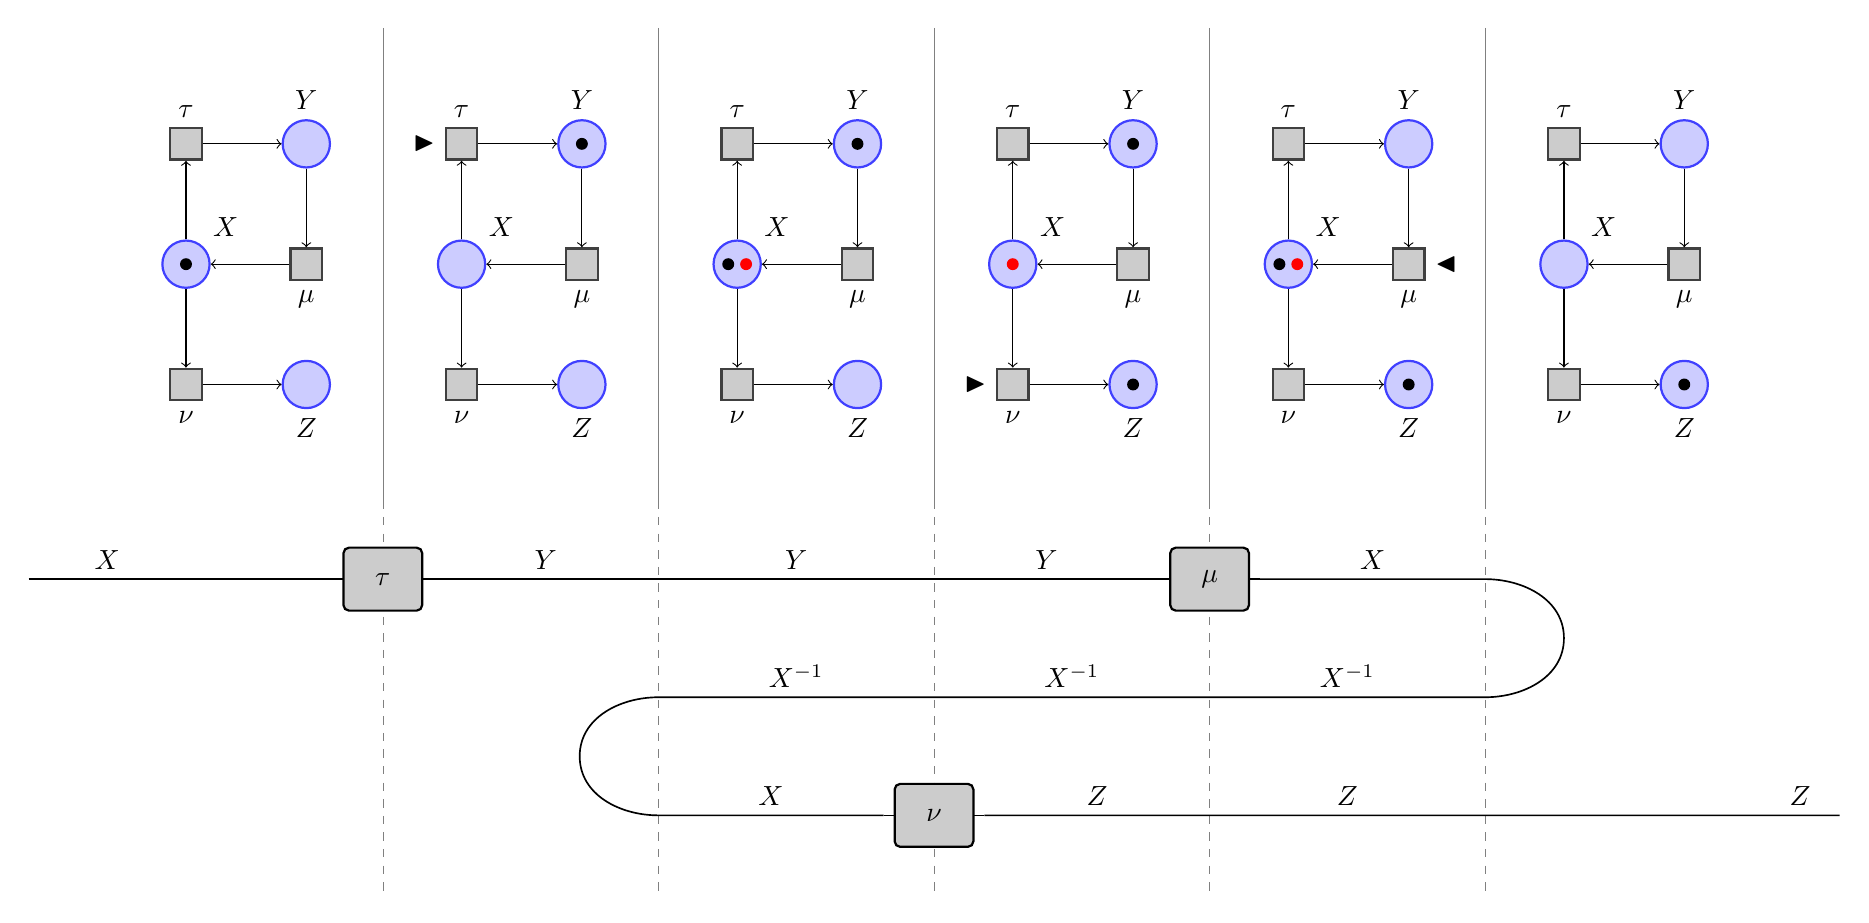
\begin{tikzpicture}
	\pgfmathsetmacro\bS{3.5}
	\pgfmathsetmacro\hkX{(\bS/3.5)}
	\pgfmathsetmacro\kY{-1.5}
	\pgfmathsetmacro\hkY{\kY*0.5}
	
	\draw pic (m0) at (0,0) {netA={{black}/{}/{}/{}/{}/{}}};
	\draw pic (m1) at (\bS,0) {netA={{}/{black}/{}/{$\blacktriangleright$}/{}/{}}};
	\draw pic (m2) at ({2 * \bS},0) {netA={{black,red}/{black}/{}/{}/{}/{}}};
	\draw pic (m3) at ({3 * \bS},0) {netA={{red}/{black}/{black}/{}/{}/{$\blacktriangleright$}}};
	\draw pic (m4) at ({4 * \bS},0) {netA={{black, red}/{}/{black}/{}/{$\blacktriangleleft$}/{}}};
	\draw pic (m5) at ({5 * \bS},0) {netA={{}/{}/{black}/{}/{}/{}}};
	
	\begin{scope}[very thin]
	\foreach \j in {1,...,5} {
		\pgfmathsetmacro \k { \j * \bS - 1 };
		\draw[gray,dashed] (\k,-3) -- (\k,-8);
		\draw[gray] (\k,3) -- (\k,-3);
	}
	\end{scope}
	
	\begin{scope}[shift={(0,-4)}, oriented WD, bbx = 1cm, bby =.4cm, bb min width=1cm, bb port sep=1]
	% [,oriented WD,bbx = 1cm, bby =.5cm, bb min width=1cm,bb port length=4pt, bb port sep=1]
	
	\draw node [fill=\backgrnd,bb={1}{1}] (Tau) at (\bS - 1,0) {$\tau$};
	\draw node [fill=\backgrnd,bb={1}{1}] (Mu)  at ({4 * \bS - 1},0) {$\mu$};
	\draw node [fill=\backgrnd,bb={1}{1}] (Nu)  at ({3 * \bS - 1},{2 * \kY}) {$\nu$};
	
	\draw (-2,0) --     node[above] {$X$}       (0,0)
	--                  node[above] {}          (Tau_in1);
	
	\draw (Tau_out1) -- node[above] {$Y$}      ({2 * \bS - 1},0)
	--                  node[above] {$Y$}      ({3 * \bS - 1},0)
	--                  node[above] {$Y$}      (Mu_in1);
	
	\draw (Mu_out1) --  node[above] {$X$}      ({5 * \bS - 1},0)
	--                  node[above] {}         ({5 * \bS - 1},0)
	to[out=0, in=90]    node[above] {}         ({5 * \bS},-0.75)
	to[out=-90,in=0]    node[below] {}         ({5 * \bS - 1},{\kY})
	--                  node[above] {}         ({5 * \bS - 1},{\kY})
	--                  node[above] {$X^{-1}$} ({4 * \bS - 1},{\kY})
	--                  node[above] {$X^{-1}$} ({3 * \bS - 1},{\kY})
	--                  node[above] {$X^{-1}$} ({2 * \bS - 1},{\kY})
	to[out=-180,in=90]  node[above] {}         ({2 * \bS - 2},{2 * \kY - \hkY})
	to[out=-90,in=-180] node[above] {}         ({2 * \bS - 1},{2 * \kY})
	--                  node[above] {$X$}      (Nu_in1);
	
	\draw (Nu_out1) --  node[above] {$Z$}      ({4 * \bS - 1},{2 * \kY})
	--                  node[above] {$Z$}      ({5 * \bS - 1},{2 * \kY})
	--                  node[above] {}         ({6 * \bS - 1},{2 * \kY})
	--                  node[above] {$Z$}      ({6 * \bS},{2 * \kY});
	
	\end{scope}
\end{tikzpicture}}
\end{document}